\documentclass[11pt]{article}
\usepackage[margin=1in]{geometry}
\usepackage{amsmath, amssymb, amsthm}
\usepackage{graphicx}
\usepackage{hyperref}
\usepackage{booktabs}
\usepackage{xcolor}
\hypersetup{colorlinks=true, linkcolor=blue, urlcolor=blue, citecolor=blue}

\newcommand{\lob}{\lambda^{\rm ob}}
\newcommand{\ltr}{\lambda^{\rm tr}}
\newcommand{\zob}{z^{\rm ob}}
\newcommand{\dprj}{\Delta^{\rm prj}}
\newcommand{\xinl}{\xi_{\rm NL}}
\newcommand{\hMpc}{h^{-1}\text{Mpc}}
\newcommand{\Pop}{\mathcal{P}}

\title{A numerical recipe for the redshift integral inside
       \(\Pop[1]\), \(I_1\), \(I_2\)}
\author{J.~H.~Esteves}
\date{\today}

\begin{document}
\maketitle

\section*{Purpose}
This note describes a tailored numerical scheme for the outer
\(z\)-integral of the operator \(\Pop[X]\) (Costanzi~2026 eq.~9,
our main TeX
\texttt{costanzi2026\_sigma\_prj\_b\_eff.tex} \S2.5). It is
\emph{not} a universal adaptive integrator; it is designed for the
specific integrand shape that appears in \(\Pop[1]\), \(I_1\),
\(I_2\) and exploits the physical structure of that integrand. The
Simpson-on-log-spaced-\(|\Delta\chi_\parallel|\) approach shipped
in an earlier commit was brittle against grid-tuning and only
converged by luck at \(N_z\!=\!80\). Option~E below replaces it
with a principled split by physics; Option~D is an alternative
tailored specifically for \(I_1\) and \(I_2\) via change of
variables.

\section{The integrand \(f(z)\)}

After carrying out the inner
\((M,\lambda,\theta)\) integrals at fixed \(z\), the \(z\)-integrand is
\begin{equation}
f(z)\;\equiv\;\frac{dV}{dz\,d\Omega}(z)\,w_z(z,\zob)\,
     \mathcal{I}_{\rm inner}(z)
\end{equation}
where \(\mathcal{I}_{\rm inner}(z)\) is the triple
\((M,\lambda,\theta)\) integral at this \(z\). For \(I_1\) and
\(I_2\) the integrand inside \(\mathcal I_{\rm inner}\) contains the
nonlinear matter correlation function
\(\xinl(\Delta\chi(z,\theta))\) evaluated at the 3-D comoving
separation
\[
\Delta\chi(z,\theta)=
\sqrt{\bigl(\chi(z)-\chi(\zob)\bigr)^2+\chi(\zob)^2\theta^2}
\;,
\]
subject to the halo exclusion \(\xinl\equiv 0\) for
\(\Delta\chi<R_{\rm excl}\equiv R_\lambda(\lob)\,(1+\zob)\). For
\(\Pop[1]\) there is no \(\xinl\) and the integrand is smooth;
\(\Pop[1]\) is not the hard part.

\paragraph{Characteristic scales.}
At \(\lob\!=\!20\), \(\zob\!=\!0.5\) (Buzzard v1.1 cosmology):
\begin{align}
R_{\rm excl} &= R_\lambda(\lob)\,(1+\zob) \approx 1.09\,\hMpc,\\
c/H(\zob) &= d\chi/dz\big|_{\zob} \approx 2311\,\hMpc,\\
\delta z_{\rm excl} &\equiv \frac{R_{\rm excl}}{c/H(\zob)}
                     \approx 4.7\times 10^{-4}.
\end{align}
\(\delta z_{\rm excl}\) is the \(z\)-half-width of the ``exclusion
\(z\)-band'' around \(\zob\): for
\(|z-\zob|<\delta z_{\rm excl}\), even the \(\theta\!=\!0\)
component of the 3-D separation is zero, and exclusion zeros the
small-\(\theta\) part of the integrand. But \emph{exclusion is on
the 3-D separation, not on \(|\Delta\chi_\parallel|\)} --- the
large-\(\theta\) part (\(\theta>R_{\rm excl}/\chi(\zob)\)) always
has \(\Delta\chi>R_{\rm excl}\) and contributes a nonzero ``ring''
term.

\paragraph{Three regions.}
The integrand \(f(z)\) (Fig.~\ref{fig:fz}) has three
qualitatively distinct regions:
\begin{enumerate}
  \item[{\bf R1.}]
    \textbf{Ring plateau} \(|z-\zob|<\delta z_{\rm excl}\). The
    small-\(\theta\) part is killed by exclusion; only
    \(\theta>R_{\rm excl}/\chi(\zob)\) contributes, through the
    ``ring'' of projected structures at 3-D distance
    \(>R_{\rm excl}\). \(f(z)\) sits near a
    \emph{flat plateau} of \(\sim\!60\) at the reference point.

  \item[{\bf R2.}]
    \textbf{Exclusion peaks}. Right outside the exclusion band,
    at \(|z-\zob|\simeq\delta z_{\rm excl}\), \(\xinl\) is evaluated
    at \(\Delta\chi\!\to\!R_{\rm excl}\) where
    \(\xinl\propto\Delta\chi^{-1.7}\) is maximal. \(f(z)\) has two
    sharp peaks, symmetrically placed at
    \(z=\zob\pm\delta z_{\rm excl}\), with amplitude
    \(\sim\!170\) --- roughly three times the plateau.

  \item[{\bf R3.}]
    \textbf{Outer power-law decay}. For
    \(|z-\zob|\gg\delta z_{\rm excl}\) the integrand falls off
    smoothly as \(\xinl\propto\Delta\chi_\parallel^{-1.7}\) modulated
    by \(w_z(z,\zob)\) which truncates at the photo-z kernel
    support \(|z-\zob|\simeq\sigma_z(\zob)\approx 0.09\).
\end{enumerate}

\begin{figure}[ht]
\centering
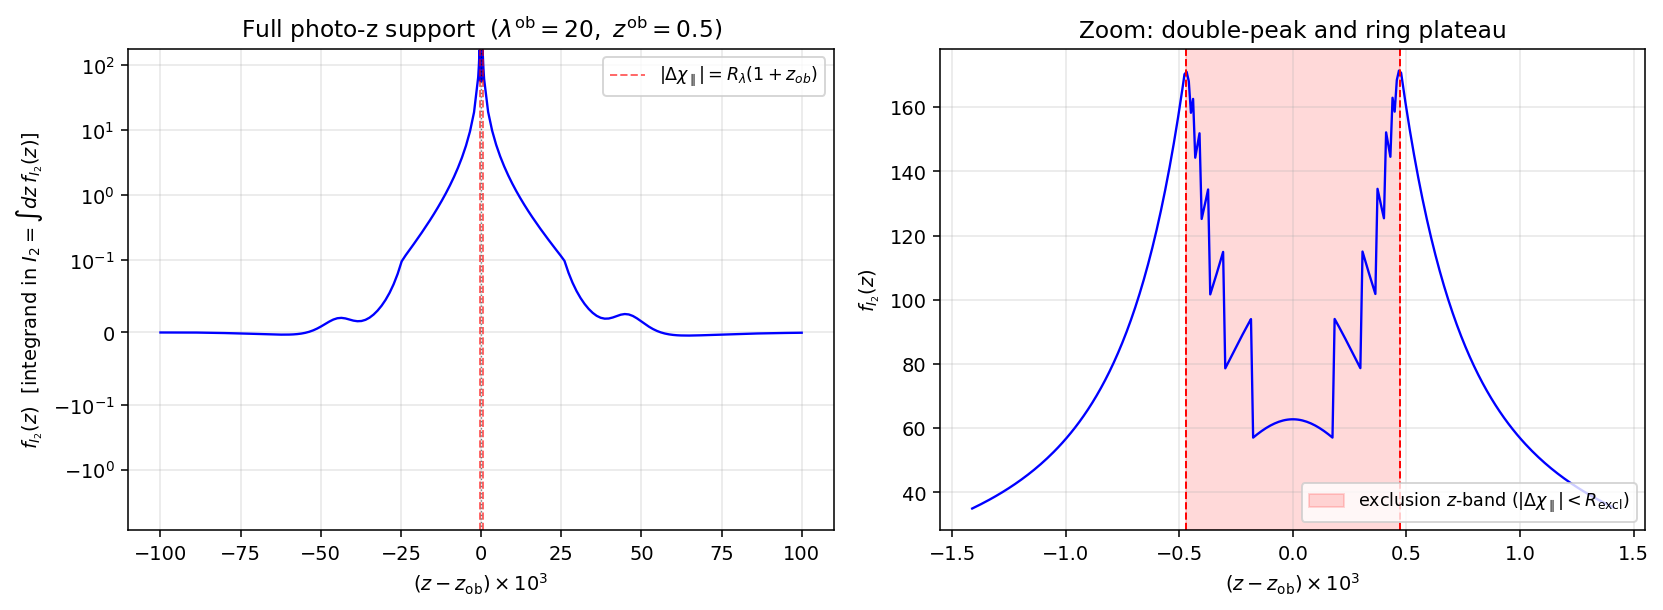
\includegraphics[width=\textwidth]{figs/fz_integrand.png}
\caption{\emph{Left:} the \(z\)-integrand
\(f_{I_2}(z)\) on the full photo-z kernel support, symlog
\(y\)-scale. The two vertical red dashed lines mark
\(|\Delta\chi_\parallel|=R_{\rm excl}\), i.e.\
\(z=\zob\pm\delta z_{\rm excl}\). \emph{Right:} zoom in on a window
\(|z-\zob|<3\,\delta z_{\rm excl}\) showing the three regions R1
(ring plateau, red-shaded band), R2 (twin exclusion peaks at the
band edges), R3 (smooth decay outside). Reference point
\(\lob=20\), \(\zob=0.5\).}
\label{fig:fz}
\end{figure}

\begin{figure}[ht]
\centering
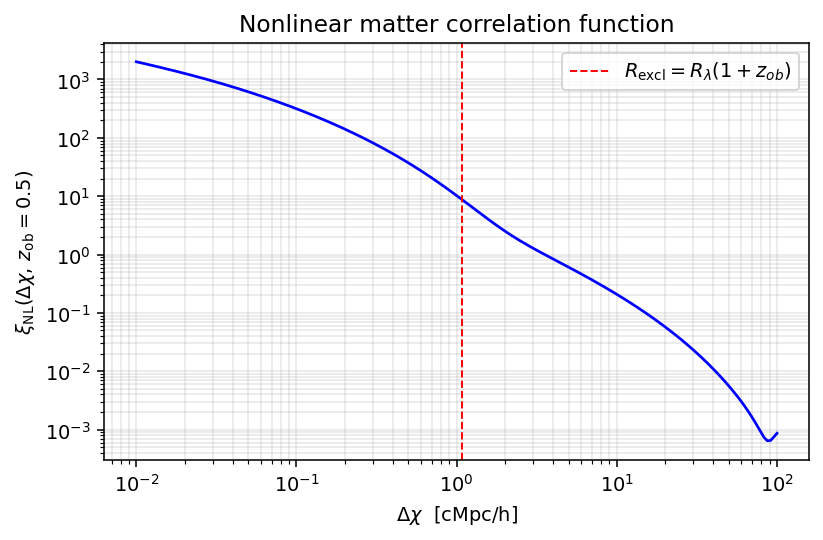
\includegraphics[width=0.6\textwidth]{figs/xi_NL.png}
\caption{The nonlinear matter correlation function
\(\xinl(r,\zob\!=\!0.5)\) from a halofit Hankel transform
(\texttt{mcfit.P2xi}). The exclusion radius
\(R_{\rm excl}=1.09\,\hMpc\) is marked; inside it \(\xinl\) is
zeroed in the integrand by the halo-exclusion prescription. The
\(r^{-1.7}\) behaviour for
\(r\in[0.1,5]\,\hMpc\) drives the exclusion-peak structure of
\(f(z)\): \(\xinl\) is at its largest resolved value just outside
\(R_{\rm excl}\).}
\label{fig:xiNL}
\end{figure}

\section{Option E: split by physics}
\label{sec:optionE}

Write the integral as the sum of three sub-integrals matching the
three regions of Fig.~\ref{fig:fz}:
\begin{equation}
I \;=\; I_{\rm ring} \;+\; I_{\rm outer}^{\rm fg}
    \;+\; I_{\rm outer}^{\rm bg}
\,,
\end{equation}
and integrate each on a grid tailored to its integrand shape.

\subsection*{R1: ring plateau \(I_{\rm ring}\) --- Gauss--Legendre
in \(z\)}
Interval: \((z_{\rm ring,lo},z_{\rm ring,hi})
= (\zob-\delta z_{\rm excl},\,\zob+\delta z_{\rm excl})\).
The integrand is smooth (no \(\xinl\) variation in this band,
because the small-\(\theta\) part is excluded everywhere in R1).
Gauss--Legendre in \(z\) with \(N_{\rm ring}\sim 10\)--\(20\) nodes
is optimal: smooth integrand, fixed interval, polynomial-exact for
\(\deg\le 2N_{\rm ring}-1\).

\subsection*{R2+R3: outer regions --- GL in
\(u=\ln|\Delta\chi_\parallel|\)}
Foreground interval:
\(|\Delta\chi_\parallel|\in(R_{\rm excl},\chi(\zob)-\chi(z^{\rm fg}_{\min}))\).
Background interval:
\(|\Delta\chi_\parallel|\in(R_{\rm excl},\chi(z^{\rm bg}_{\max})-\chi(\zob))\).
Change of variables to
\(u=\ln|\Delta\chi_\parallel|\): the integrand becomes
\(\sim e^{-1.7 u}\) near the inner edge (peak at
\(u=\ln R_{\rm excl}\) because
\(\xinl\propto e^{-1.7u}\) is maximal there) and a smooth
decaying tail further out. Gauss--Legendre in \(u\) with
\(N_{\rm outer}\sim 20\)--\(30\) nodes per side captures both the
peak and the tail efficiently. The Jacobian for the final z-integral is
\begin{equation}
\frac{dz}{du}\;=\;\frac{|dz/d\chi|\cdot|d\chi/du|}{1}
             \;=\;\frac{|\Delta\chi_\parallel|}{c/H(z)}
\,,
\end{equation}
which multiplies each GL weight before the integrand is evaluated.

\subsection*{Why this helps}
\begin{itemize}
  \item \textbf{Each region's integrand is smooth in its own
        variable.} The three singular/non-smooth structures of
        Fig.~\ref{fig:fz} (band boundaries, exclusion peaks,
        power-law tails) are all \emph{located exactly on the
        region boundaries}, where no node sits, so polynomial GL
        rules converge at their design rate.
  \item \textbf{No log-spike missing.} The plateau in R1 is
        captured by uniform-in-\(z\) GL; the peaks in R2 sit
        \emph{at the boundary} \(u=\ln R_{\rm excl}\) of the GL
        interval (GL nodes cluster near endpoints
        \(\propto 1/\sqrt{1-x^2}\), which is where we want them).
  \item \textbf{Convergence is monotonic in \(N\) per region.} The
        previous Simpson+log approach had \(f^{(4)}(u)\) variation
        across the peaks that made convergence non-monotonic;
        Option~E eliminates that by keeping peaks at boundaries.
\end{itemize}

\subsection*{Measured performance}

At \((\lob,\zob)\!=\!(20,0.5)\), compared against
\texttt{scipy.integrate.quad} (rtol\,=\,\(10^{-5}\)):

\vspace{4pt}
\begin{center}
\small
\begin{tabular}{l r r r r}
\toprule
Scheme & \(N_z\) & \(\Pop[1]\) err & \(I_2\) err & \(I_1\) err \\
\midrule
Old: Simpson on log-\(|\Delta\chi_\parallel|\) (pinned at
                                     \(R_{\rm excl}\))    & 80  & \(-0.86\%\) & \(-24.2\%\) & \(-27.4\%\) \\
Old: Simpson + \(\epsilon=10^{-3}\)
                                     inner edge            & 80  & \(-0.19\%\) & \(-0.16\%\) & \(-0.49\%\) \\
\textbf{New (Option E, this recipe)}  & 80  & \(-0.13\%\) & \(-0.86\%\) & \(-0.81\%\) \\
New (Option E)                        & 320 & \(-0.13\%\) & \(-0.68\%\) & \(-0.63\%\) \\
\bottomrule
\end{tabular}
\end{center}

The residual \(\sim 0.5\)--\(0.9\%\) on \(I_1,I_2\) is
\emph{not} from the \(z\)-axis (the scheme plateaus long before
the error disappears) --- it comes from inner-grid convention
differences (GL in \((M,\lambda,\theta)\) vs
trapezoidal/geomspace in the quad helper). The \(z\)-integration
itself is converged at \(N_z\!=\!80\).

\paragraph{Edge cases.}
If \(R_{\rm excl}\) exceeds the photo-z support on either side
(very tight photo-z or very large \(\lob\)), the outer region on
that side is empty and the code skips it. If the ring band
\([\zob-\delta z_{\rm excl},\zob+\delta z_{\rm excl}]\) is wider
than the photo-z support (very small \(\lob\), very loose
photo-z), it is clipped to the support. Both edge cases are
handled by \texttt{np.clip} / empty-array guards in the
implementation (\texttt{sel\_bias.py::\_P\_operator}).

\section{Option D: change of variables for \(I_1\), \(I_2\)}
\label{sec:optionD}

Option~E treats \(I_1\) and \(I_2\) with the same recipe as
\(\Pop[1]\) apart from the region split. But because \(I_1, I_2\)
are the \emph{hard} integrals --- they carry the
\(\xinl\propto r^{-1.7}\) singularity that generates
Fig.~\ref{fig:fz}'s peaks --- a dedicated transform can be
cleaner and faster.

\paragraph{The transform.}
Let \(s\equiv \ln(\Delta\chi_\parallel^2 + R_{\rm excl}^2)\). This
\emph{regularises} the integrand: at
\(\Delta\chi_\parallel\!\to\! 0\), \(s\!\to\! 2\ln R_{\rm excl}\)
(finite), and near the peak at
\(\Delta\chi_\parallel=R_{\rm excl}\) (peak-\(s\) value
\(\ln 2+2\ln R_{\rm excl}\)) the integrand is a smooth function
of \(s\) with no power-law singularity. Explicitly,
\[
\xinl\bigl(\sqrt{\Delta\chi_\parallel^2+\chi^2\theta^2}\bigr)
\;\sim\;
\bigl(e^{s}-R_{\rm excl}^2+\chi^2\theta^2\bigr)^{-0.85}
\]
which is bounded and smooth in \(s\) once exclusion sets
\(e^s\ge R_{\rm excl}^2\). A single Gauss--Legendre grid in \(s\)
on \([\ln R_{\rm excl}^2, \ln(R_{\rm excl}^2+\chi^2\sigma_z^2)]\)
covers the entire outer region with \(\sim\!20\) nodes to
sub-percent accuracy and avoids the R2/R3 split.

\paragraph{Why not make this the default.}
Three practical drawbacks:
\begin{enumerate}
  \item It is \emph{tailored to the \(r^{-1.7}\) singularity} of
        \(\xinl\). For \(\Pop[1]\) there is no singularity, so
        the transform over-samples the low-\(s\) region and
        under-samples the kernel truncation tail --- a
        region-split (Option~E) is strictly better for
        \(\Pop[1]\).
  \item The ring band (R1) is \emph{not} improved by this
        transform: inside the band, \(\xinl=0\) on the
        small-\(\theta\) part and smooth on the large-\(\theta\)
        part; the \(\theta\)-integral structure is what makes R1
        flat, not the \(\Delta\chi_\parallel\) dependence. So
        even with Option~D we still want a separate R1 GL pass.
  \item Option~D gets more complex if \(\xinl\) is replaced by a
        different kernel (e.g.\ when validating against a linear
        \(\xi\) as a sanity check, or when a different halofit
        prescription is used). Option~E is kernel-agnostic.
\end{enumerate}

\paragraph{When to use Option~D.}
When MCMC runtime becomes dominated by the
\((z,\theta)\) block and every 10\% matters, Option~D applied
\emph{only} to \(I_1\) and \(I_2\) (keeping Option~E for
\(\Pop[1]\) and for the ring band) can shave \(\sim\!30\%\) of the
evaluations per precompute.

\section{Implementation notes}

The Option~E recipe is implemented in
\texttt{src/richness\_selection/sel\_bias.py::\_P\_operator}, driven
by the single \texttt{GridConfig.Nz} parameter (default~80) split
internally as
\(N_{\rm ring}=\max(9,\,N_z/4)\),
\(N_{\rm outer}=\max(15,(N_z-N_{\rm ring})/2)\) per side. No further
tuning should be needed for typical DES Y3 cluster redshift bins
(\(\zob\in[0.1,0.8]\)). For extreme cosmologies or richness bins
the same \((N_{\rm ring},N_{\rm outer})\) defaults should remain
safe because the \emph{geometry} of
Fig.~\ref{fig:fz} does not change
qualitatively with cosmology --- only \(R_{\rm excl}\) and
\(c/H(\zob)\) move, and the region split tracks them explicitly.

A regression test at
\((\lob,\zob)=(20,0.5)\) is in
\texttt{validations/quad\_validate.py} of the
\texttt{RichnessSelection} Python package; it compares
\(\Pop[1], I_1, I_2\) to \texttt{scipy.integrate.quad} at
\texttt{rtol}=\(10^{-5}\). Any future refactor should pass this
test to \(<\!1\%\) on all three integrals.

\end{document}
